\section{Appendix}
\label{sec: AppendixA}

The reduction of the Wendling model is based on the principles of linear superposition. First notice that each synapse is a linear lowpass filter (equation~\ref{eqn: LaplaceNMM}). In figure~\ref{fig: Biological} there are eight such synapse. However, notice that numerous of these synapse have identical synaptic gains, and are connected by different connectivity constants. Given that for a linear system it is known that
\begin{align}
f(a\mathbf{x}) = af(\mathbf{x}),
\end{align} where $f(\cdot)$ is an arbitrary function, and $a$ is a constant. Therefore, the model can be simplified by moving the synapse closer to the respective populations. The result of this process is demonstrated in figure~\ref{fig: BiologicalMin}.

\begin{figure}  %%%%%%%%%%%%%%%%%%%%%%%%%%%%%%%%%%%%%%%
	\centering
		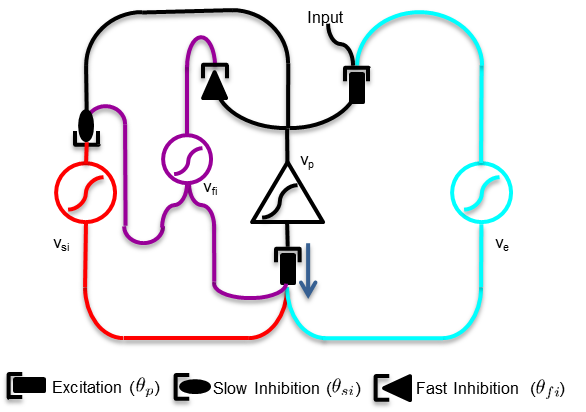
\includegraphics{Biological_Model_DescriptionMin.png}
	\caption{Graphical Description of the Wendling model (Minimised). Membrane potentials are shown and named $v_{b}$ where $b$ is $p$, $e$, $fi$ and $si$ for pyramidal, excitatory and slow and fast inhibitory populations, respectively. The synaptic gains of each population are specified by $\theta_{m}$ where $m$ is defined in the same manner as the membrane potentials and $\theta_{p}=\theta_{e}$. Each triangle and circle indicates a neural population. In particular, the triangle shape indicates the pyramidal population and the circle shapes represent interneurons. The triangles and circles model the action of the soma for the neural populations, and convert membrane potentials to firing rates. The synapses convert the firing rates to membrane potentials. Lastly, each line indicates a neural connection, which is specified by a connectivity constant.}
	\label{fig: BiologicalMin}
\end{figure}%%%%%%%%%%%%%%%%%%%%%%%%%%%%%%%%%%%%%%%%%%%%%

Now consider the full set of original model equations that would be required to specify figure~\ref{fig: Biological}
\begin{align}
\label{eqn: Fullmodel Descrip}
\mathrm{d}v_{po*}(t)&= z_{po*}(t)\mathrm{d}t\\
\mathrm{d}z_{po*}(t)&=\left(\frac{\theta_{p}(t)}{\tau_{p}}c_{1}g(v_{p}(t))-2\frac{z_{po*}(t)}{\tau_{p}}-\frac{v_{po*}(t)}{\tau_{p}^{2}}\right)\mathrm{d}t\\
\mathrm{d}v_{p1*}(t)&= z_{p1*}(t)\mathrm{d}t\\
\mathrm{d}z_{p1*}(t)&=\left(\frac{\theta_{p}(t)}{\tau_{p}}c_{3}g(v_{p}(t))-2\frac{z_{p1*}(t)}{\tau_{p}}-\frac{v_{p1*}(t)}{\tau_{p}^{2}}\right)\mathrm{d}t\\
\mathrm{d}v_{p2*}(t)&= z_{p2*}(t)\mathrm{d}t\\
\label{eqn: Pyr}
\mathrm{d}z_{p2*}(t)&=\left(\frac{\theta_{p}(t)}{\tau_{p}}c_{5}g(v_{p}(t))-2\frac{z_{p2*}(t)}{\tau_{p}}-\frac{v_{p2*}(t)}{\tau_{p}^{2}}\right)\mathrm{d}t\\
\label{eqn: SI}
\mathrm{d}v_{p3*}(t)&= z_{p3*}(t)\mathrm{d}t\\
\mathrm{d}z_{p3*}(t)&=\left(\frac{\theta_{si}(t)}{\tau_{si}}c_{4}g(v_{si}(t))-2\frac{z_{p3*}(t)}{\tau_{si}}-\frac{v_{p3*}(t)}{\tau_{si}^{2}}\right)\mathrm{d}t\\
\mathrm{d}v_{p4*}(t)&= z_{p4*}(t)\mathrm{d}t\\
\label{eqn: SI1}
\mathrm{d}z_{p4*}(t)&=\left(\frac{\theta_{si}(t)}{\tau_{si}}c_{6}g(v_{si}(t))-2\frac{z_{p4*}(t)}{\tau_{si}}-\frac{v_{p4*}(t)}{\tau_{si}^{2}}\right)\mathrm{d}t\\
\label{eqn: FI}
\mathrm{d}v_{p5*}(t)&= z_{p5*}(t)\mathrm{d}t\\
\label{eqn: FI2}
\mathrm{d}z_{p5*}(t)&=\left(\frac{\theta_{fi}(t)}{\tau_{fi}}c_{7}g(v_{fi}(t))-2\frac{z_{p4*}(t)}{\tau_{fi}}-\frac{v_{p5*}(t)}{\tau_{fi}^{2}}\right)\mathrm{d}t\\
\label{eqn: Exc}
\mathrm{d}v_{p6*}(t)&= z_{p6*}(t)\mathrm{d}t\\
\mathrm{d}z_{p6*}(t)&=\left(\frac{\theta_{e}(t)}{\tau_{e}}c_{2}g(v_{e}(t))-2\frac{z_{p6*}(t)}{\tau_{e}}-\frac{v_{p6*}(t)}{\tau_{e}^{2}}\right)\mathrm{d}t\\
\mathrm{d}v_{p7*}(t)&= z_{p7*}(t)\mathrm{d}t\\
\label{eqn: WienerFull}
\mathrm{d}z_{p7*}(t)&=\left(\frac{\theta_{p}(t)}{\tau_{p}}\mu -2\frac{z_{p7*}(t)}{\tau_{e}}-\frac{v_{p7*}(t)}{\tau_{p}^{2}}\right)\mathrm{d}t + \frac{\theta_{p}(t)}{\tau_{p}}\epsilon(t)\mathrm{d}W.\\
\end{align} In these equations $dW$ represents a Wiener process and is required as $\epsilon(t)\sim N(0,\sigma)$, where $\sigma$ and $\mu$ (equation~\ref{eqn: Wiener}) describe the mean and variance of the stochastic model input. Further, $v_{po}(t) $ and $v_{p1-7*}(t)$ represent the membrane potential produced by each synapse and $z_{po*}(t) $ and $z_{p1-7*}(t)$ their derivatives. The inputs to each neural population are specified by $v_{b}(t) $ and $z_{b}(t) $, and are the membrane potential of the specific population, where $b$ takes the values of $p$, $e$, $fi$ and $si$ representing pyramidal, excitatory, and slow and fast inhibitory populations, respectively. Therefore $v_{p}(t) $ is the output of the model. All $v_{b}(t) $ can be described in terms of $v_{po}(t)$ and $v_{p1-7}(t)$ as follows
\begin{align}
\label{eqn: pop1}
v_{p}(t) &= v_{p6*}(t)+v_{p7*}(t)-v_{p3*}(t)-v_{p5*}(t)\\
\label{eqn: pop2}
v_{e}(t) &= v_{po*}(t)\\
\label{eqn: pop3}
v_{si}(t) &= v_{p1*}(t)\\
\label{eqn: pop4}
v_{fi}(t) &= v_{p2*}(t)-v_{p4*}(t).
\end{align} Notice that equations~\ref{eqn: Fullmodel Descrip}-\ref{eqn: Pyr} and equations~\ref{eqn: SI}-\ref{eqn: SI1} are identical except for the connectivity constants. Further, in this model it is assumed that 
\begin{align}
\theta_p = \theta_e\\
\tau_p = \tau_e.
\end{align} Therefore, equations~\ref{eqn: Exc}-\ref{eqn: WienerFull} are identical, but have different inputs. Next consider the effect of the states $v_{p0-7*}(t)$ and $z_{p0-7*}(t)$ on the model inputs. Note that since the effect of $v_{p6*}(t)$ and $v_{p7*}(t)$ are additive, they can be added prior to being passed through the linear filter since
\begin{align}
f{x} + f{y} = f{x+y},
\end{align} where f is defined above and $x$ and $y$ are arbitrary variables. Therefore equations~\ref{eqn: Exc}-\ref{eqn: WienerFull} can be simplified to the following:
\begin{align}
\mathrm{d}v_{p1}(t)&= z_{p1}(t)\mathrm{d}t\\
\label{eqn: Wiener1}
\mathrm{d}z_{p1}(t)&=\left(\frac{\theta_{e}(t)}{\tau_{e}}(\mu +n_{e}g(v_{e}(t))-2\frac{z_{p1}(t)}{\tau_{e}}-\frac{v_{p1}(t)}{\tau_{e}^{2}}\right)\mathrm{d}t + \frac{\theta_{e}(t)}{\tau_{e}}\epsilon(t)\mathrm{d}W.
\end{align}. By making this reduction the effect of both the excitatory population and the input have been incorporated in one potential. Therefore, $v_{p7*}(t)$ is no longer required in equations~\ref{eqn: pop1}. 

Next consider the equations that only have connectivity constants that are different. Notice that these connectivity constants scale the input to the function, and this scaling can be performed after the input is transformed by the linear function. Therefore, equations~\ref{eqn: Fullmodel Descrip}-\ref{eqn: Pyr} can be represented by a single equation such that
\begin{align}
\mathrm{d}v_{po}(t)&= z_{po}(t)\mathrm{d}t\\
\mathrm{d}z_{po}(t)&=\left(\frac{\theta_{p}(t)}{\tau_{p}}g(v_{p}(t))-2\frac{z_{po}(t)}{\tau_{p}}-\frac{v_{po}(t)}{\tau_{p}^{2}}\right)\mathrm{d}t.
\end{align} Notice that in doing this equations~\ref{eqn: pop2}-\ref{eqn: pop4} are no longer valid and need to be altered to include the connectivities that have been removed from their relevant functions
\begin{align}
\label{eqn: pop2n}
v_{e}(t) &= c_{1}v_{po}(t)\\
\label{eqn: pop3n}
v_{si}(t) &= c_{3}v_{p0}(t)\\
\label{eqn: pop4n}
v_{fi}(t) &= c_{5}v_{p0}(t)-v_{p4*}(t).
\end{align}. 

A similar argument can be applied to equations~\ref{eqn: SI}-\ref{eqn: SI1} which can be simplified to
\begin{align}
\mathrm{d}v_{p2}(t)&= z_{p2}(t)\mathrm{d}t\\
\mathrm{d}z_{p2}(t)&=\left(\frac{\theta_{si}(t)}{\tau_{si}}g(v_{si}(t))-2\frac{z_{p2}(t)}{\tau_{si}}-\frac{v_{p2}(t)}{\tau_{si}^{2}}\right)\mathrm{d}t.
\end{align} Again by doing so equation~\ref{eqn: pop1} and~\ref{eqn: pop4n} are no longer valid and become
\begin{align}
v_{p}(t) &= v_{p1}(t)-c_{4}v_{p2}(t)-v_{p5*}(t)\\
v_{fi}(t) &= c_{5}v_{p0}(t)-c_{6}v_{p2}(t).
\end{align}. Lastly for simplicity equations~\ref{eqn: FI}-\ref{eqn: FI2} are replaced with
\begin{align}
\mathrm{d}v_{p3}(t)&= z_{p3}(t)\mathrm{d}t\\
\label{eqn: FI1}
\mathrm{d}z_{p3}(t)&=\left(\frac{\theta_{fi}(t)}{\tau_{fi}}c_{7}g(v_{fi}(t))-2\frac{z_{p3}(t)}{\tau_{fi}}-\frac{v_{p3}(t)}{\tau_{fi}^{2}}\right)\mathrm{d}t.
\end{align} Which results in the set of equations demonstrated in the methods section. Notice that the $n_{b}$ term used in the general form of the equations specifies connectivities that were not removed from the full model description equations due to simplification.

